%! Author = alida
%! Date = 20/11/2024

% Preamble
\documentclass[@SRC@/main]{subfiles}
\graphicspath{{@IMAGES@}}
% tutti i pacchetti usati vanno nel main

% Document
\begin{document}
    \vspace{1.5 pt}

    \clearpage


    \section{Analisi}

    \subsection{Fit calibrazione}
    Le misure di calibrazione evidenziano il corretto funzionamento degli
    strumenti, i quali forniscono misure di corrente coerenti tra loro. In seguito
    si riporta la regressione lineare effettuata sui dati in Tabella~\ref{tab:fit-calibrazione}.
    \vspace{0.75cm}
    \begin{center}
        \begin{minipage}{.8\textwidth}
            \centering
            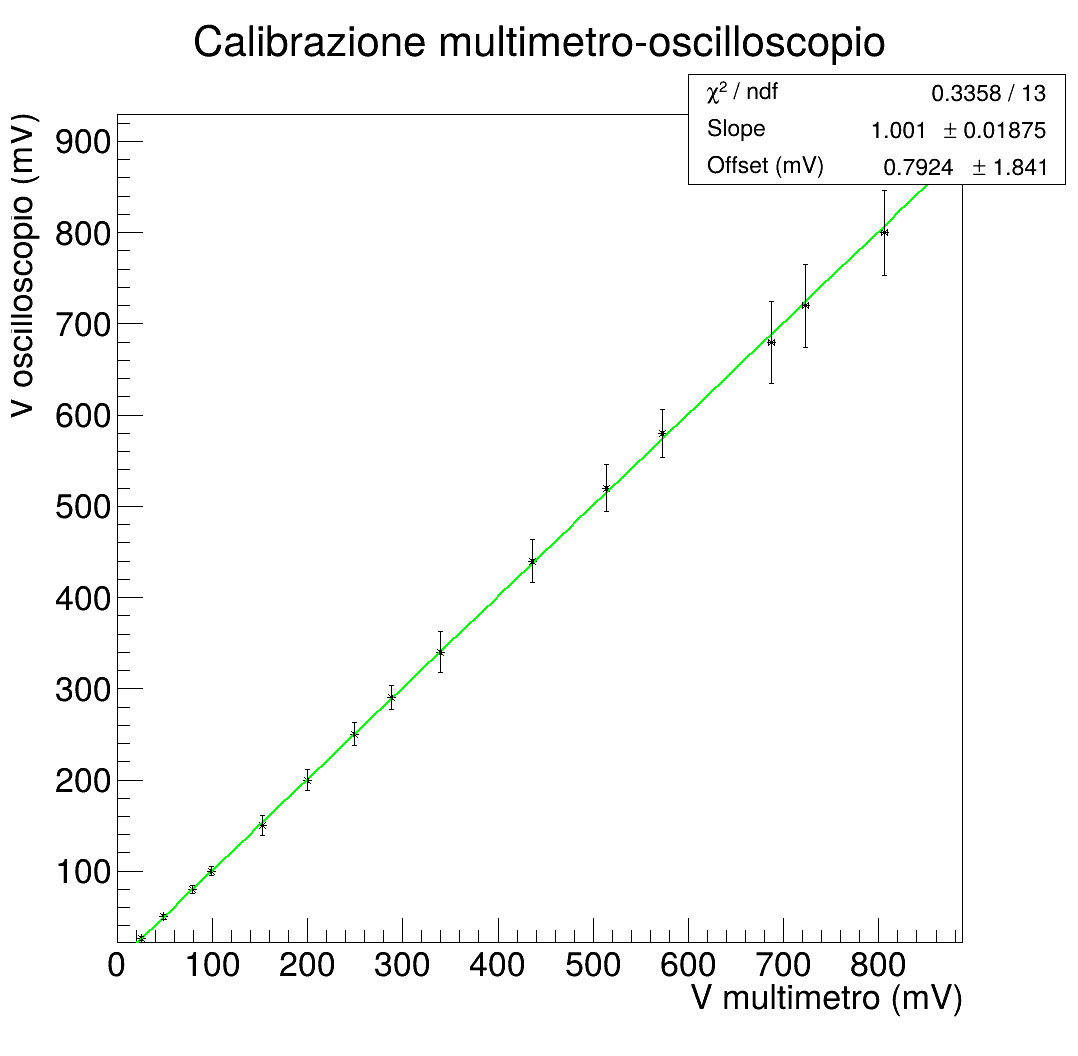
\includegraphics[width=.75\textwidth]{calibrazione.png}
            \captionof{figure}{Grafico e fit dei valori ottenuti dalla misura di calibrazione.}
            \label{fig:calibrazione}
        \end{minipage}
    \end{center}

    \vspace{5pt}
    \noindent Il fit lineare sui dati di calibrazione (Tabella~\ref{tab:calibrazione})
    fornisce le seguenti stime di coefficiente angolare e intercetta:

    \vspace{0.25cm}
    \begin{center}
        \begin{minipage}{.95\textwidth}
            \centering
            \begin{tabular}{||c|c||}
                \hline
                Pendenza          & Intercetta (mV) \\
                \hline
                $1.001 \pm 0.019$ & $0.8 \pm 1.8$   \\
                \hline
            \end{tabular}
            \captionof{table}{Risultati del fit sui dati di calibrazione.}
            \label{tab:fit-calibrazione}
        \end{minipage}
    \end{center}
    \vspace{0.25cm}
    I parametri stimati dal fit lineare, riportati in Tabella~\ref{tab:fit-calibrazione},
    sono compatibili, entro gli errori, con i valori attesi: rispettivamente 1 e 0.
    \vspace{0.1cm}

    \subsection{Fit caratteristiche}
    Nella fase di analisi sono stati effettuati due fit distinti sui dati delle curve
    caratteristiche (Tabelle~\ref{tab:silicio}~e~\ref{tab:germanio}).
    Nel primo fit è stata utilizzata la relazione eq\,\eqref{eq:caratteristiche}, nel secondo sono stati convertiti i dati in
    scala semi-logaritmica e la funzione utilizzata per il fit diventa:
    \vspace{0.5cm}
    \begin{equation*}
        \ln  (I(V_D)) = \ln \left( I_0 \cdot \exp^{\frac{V_D}{\eta V_T}} \right) \implies
        I_{ln}(V_D) = \frac{1}{\eta V_T} \cdot V_D + \ln (I_0)
    \end{equation*}
    \newpage
    \noindent Si è deciso di presentare due stime delle quantità $I_{0}$ e $\eta V_{T}$
    in quanto il fit in scala semi-logaritmica
    permette l'utilizzo di una regressione lineare, in grado di stimare i parametri del fit in modo analitico e
    pertanto
    generalmente più preciso del metodo del minimo $\chi^2$, calcolato numericamente.
    Si veda l'appendice~\ref{subsec:propagazione-errori-log} per la propagazione degli
    errori in scala semi-logaritmica.
    \vspace{4pt}
    \newline
    \begin{center}
        \begin{minipage}{.95\textwidth}
            \centering
            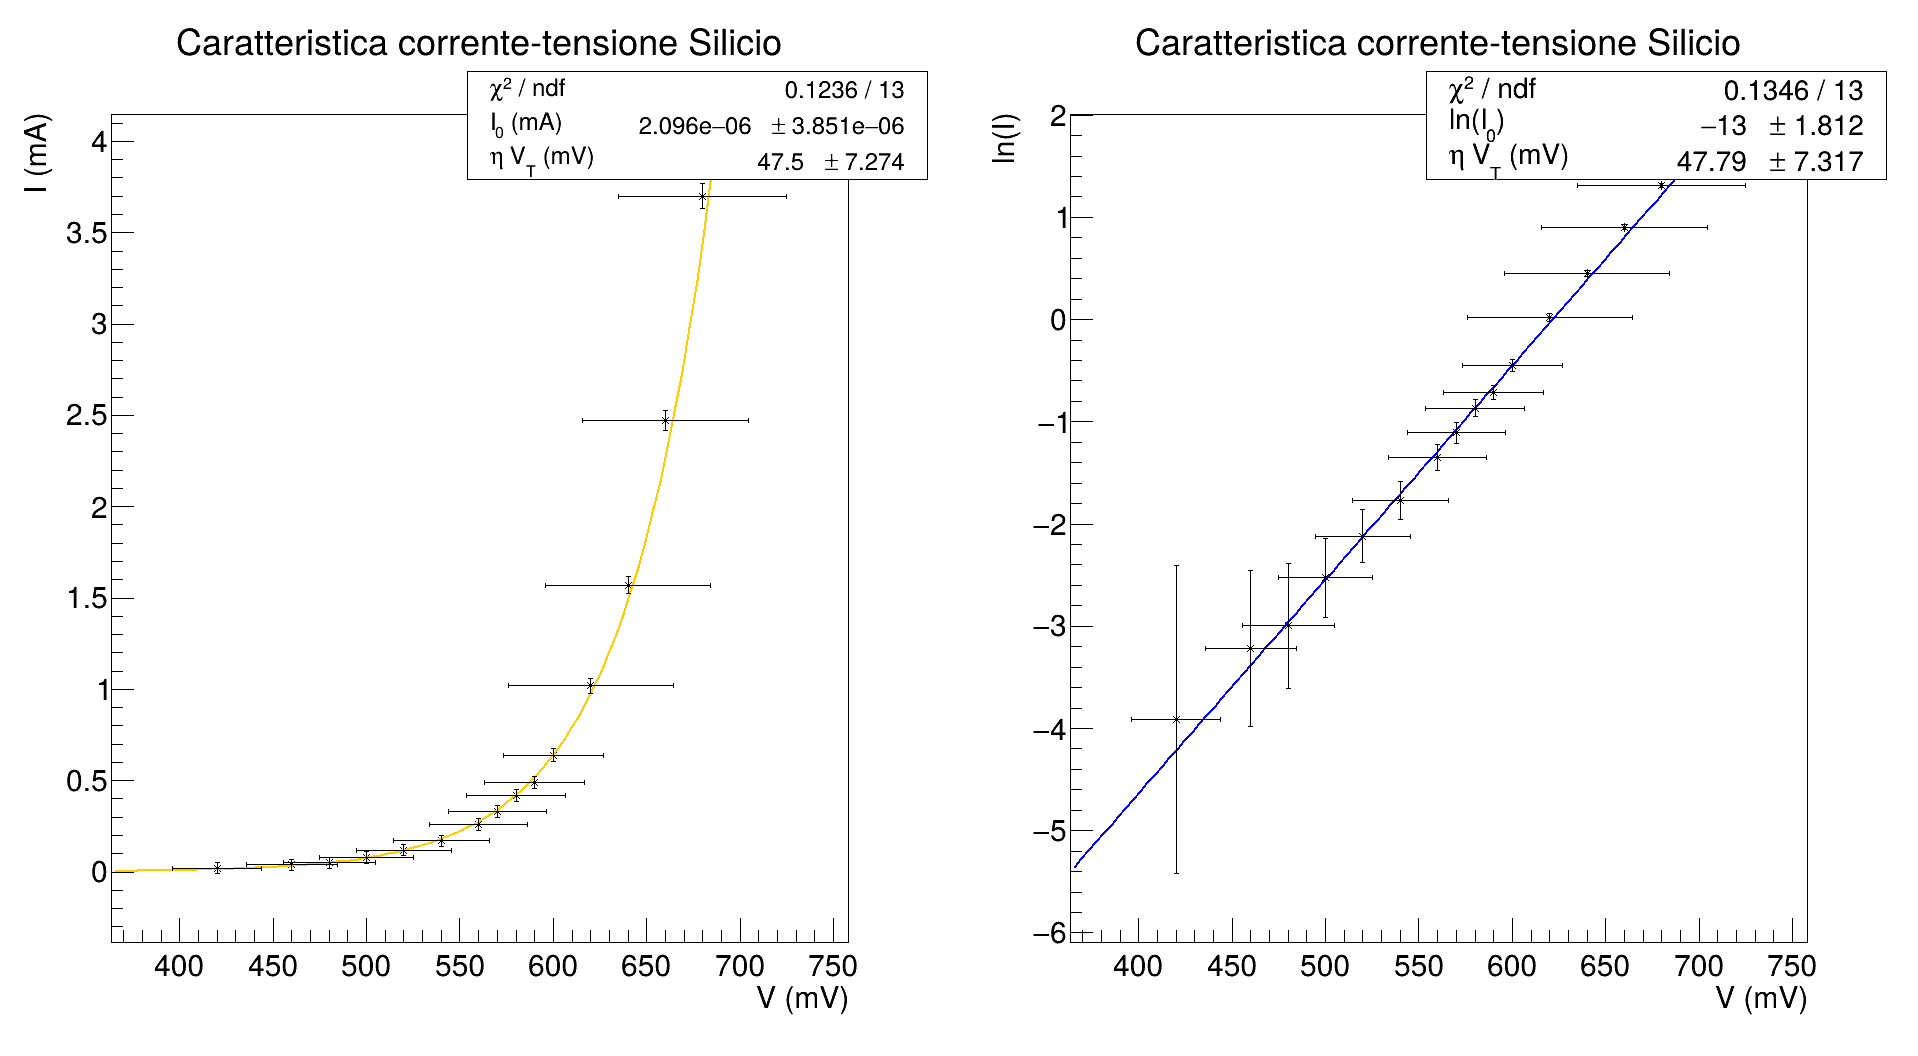
\includegraphics[width=\textwidth]{silicio.png}
            \captionof{figure}{Grafici e fit dei valori ottenuti dalla misura della caratteristica del diodo al Silicio:
            in scala lineare (destra), in scala semi-logaritmica (sinistra).}
            \label{fig:silicio}
        \end{minipage}
    \end{center}
    \vspace{0.5pt}
    \begin{center}
        \begin{minipage}[t]{.95\textwidth}
            \centering
            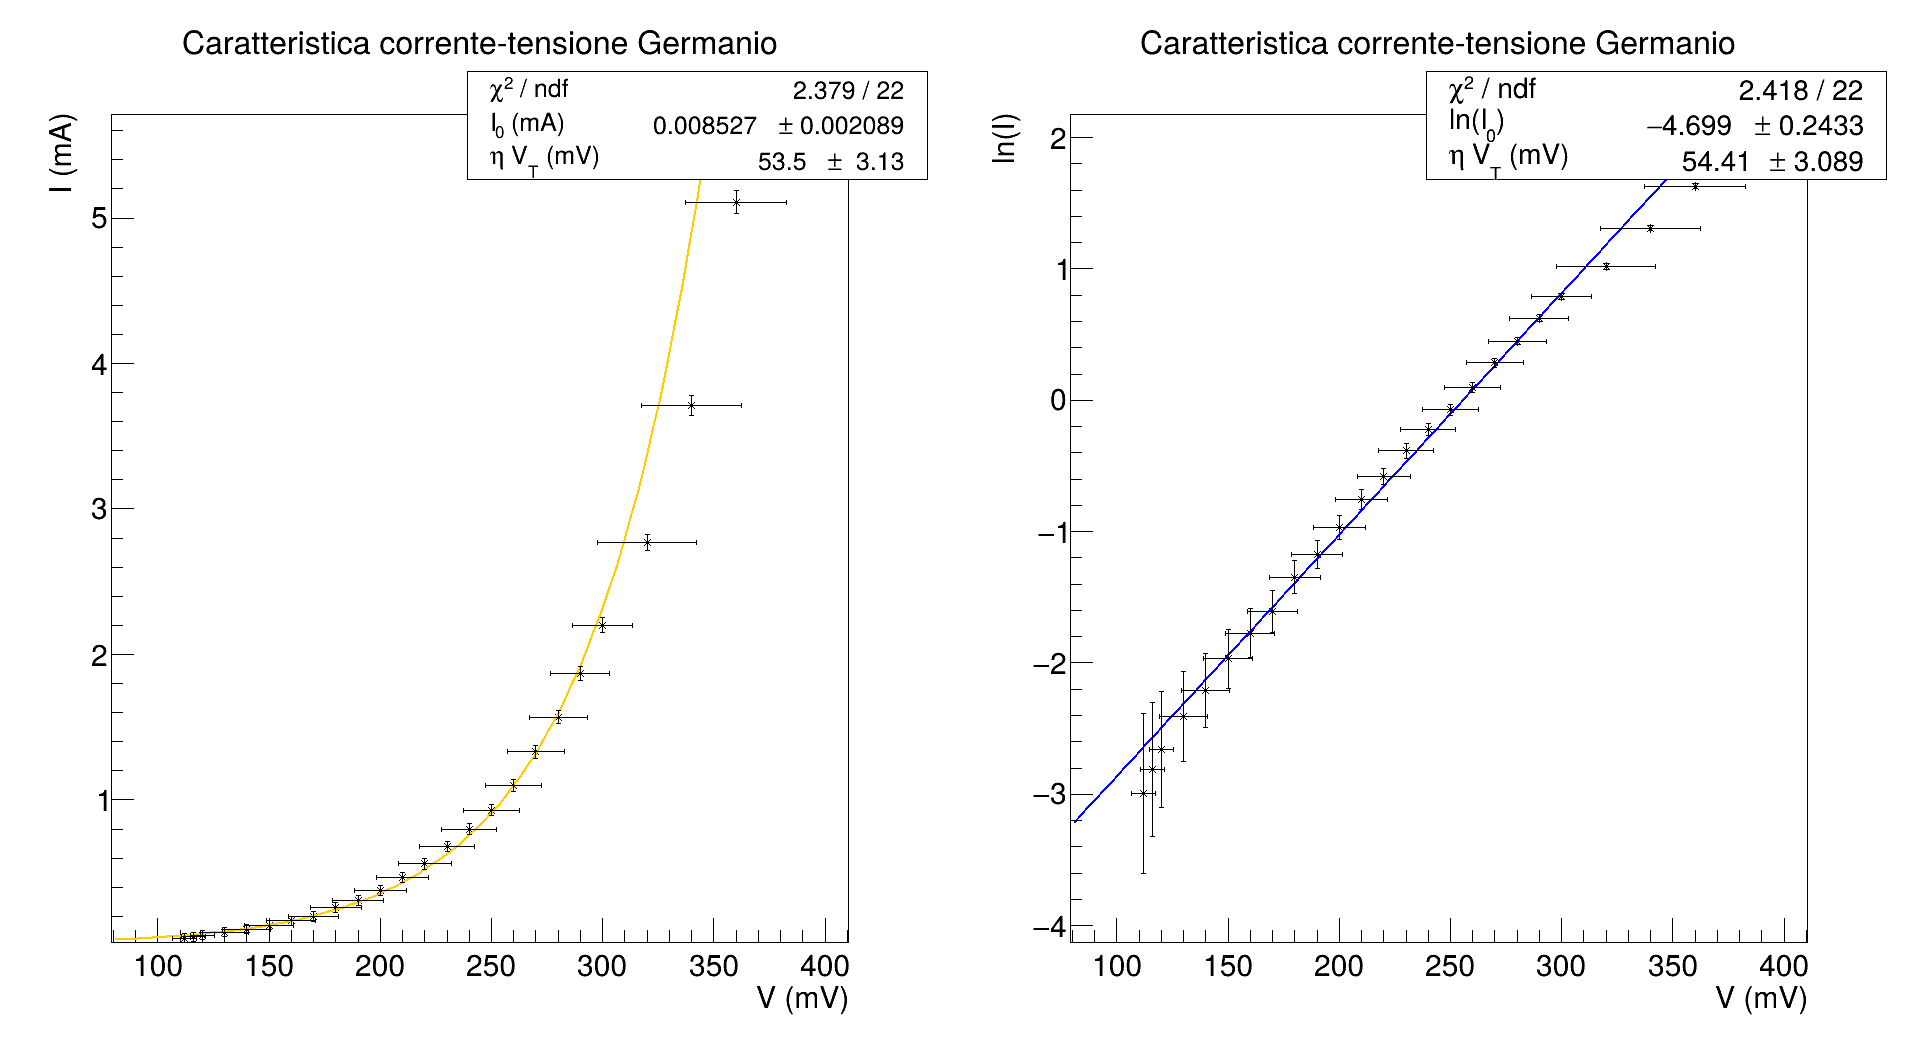
\includegraphics[width=\textwidth]{germanio.png}
            \captionof{figure}{Grafici e fit dei valori ottenuti dalla misura della caratteristica del diodo al Germanio:
            in scala lineare (destra), in scala semi-logaritmica (sinistra).}
            \label{fig:germanio}
        \end{minipage}
    \end{center}
    \vspace{1.5cm}

    \noindent I fit effettuati, riportati nelle Figure~\ref{fig:silicio} e~\ref{fig:germanio}, restituiscono i valori:
\vspace{0.2cm}
%    \begin{table}[ht]
%        \centering
%        \begin{subtable}{.45\textwidth}
%            \centering
%            \begin{tabular}{||c|c|c||}
%                \hline
%                \multicolumn{3}{||c||}{Silicio} \\
%                \hline
%                Scala            & $I_0$ (\textnormal{A})       & $\eta V_T$ (\textnormal{mV}) \\
%                \hline
%                lineare          & $(2.1\pm3.9)\cdot 10^{-9}$   & $47.5\pm7.3$                 \\
%                \hline
%                semi-logaritmica & $(2.3 \pm 4.1)\cdot 10^{-9}$ & $47.8\pm 7.3$                \\
%                \hline
%            \end{tabular}
%            \caption{Silicio}
%            \label{tab:fit-silicio}
%        \end{subtable}
%        \hfill
%        \begin{subtable}{.45\textwidth}
%            \centering
%            \begin{tabular}{||c|c|c||}
%                \hline
%                \multicolumn{3}{||c||}{Germanio} \\
%                \hline
%                Scala            & $I_0$ (\textnormal{A})       & $\eta V_T $ (\textnormal{mV}) \\
%                \hline
%                lineare          & $(8.5\pm2.1) \cdot 10^{-6}$  & $53.5\pm3.1$                  \\
%                \hline
%                semi-logaritmica & $(9.1\pm 2.2) \cdot 10^{-6}$ & $54.4\pm3.1$                  \\
%                \hline
%            \end{tabular}
%            \caption{Germanio}
%            \label{tab:fit-germanio}
%        \end{subtable}
%        \caption{Risultati dei fit effettuati sulle misure delle caratteristiche dei due diodi}
%        \label{tab:fit-diodi}
%    \end{table}

    \begin{table}[ht]
        \centering
        \begin{tabular}{||c|c|c||}
            \hline
            \multicolumn{3}{||c||}{Silicio} \\
            \hline
            Scala            & $I_0$ (\textnormal{A})       & $\eta V_T$ (\textnormal{mV}) \\
            \hline
            lineare          & $(2.1\pm3.9)\cdot 10^{-9}$   & $47.5\pm7.3$                 \\
            \hline
            semi-logaritmica & $(2.3 \pm 4.1)\cdot 10^{-9}$ & $47.8\pm 7.3$                \\
            \hline
        \end{tabular}
        \caption{Risultati dei fit effettuati sulle misure delle caratteristiche del diodo
        al Silicio. Sono riportate anche le incertezze associate alle misure, calcolate in
        appendice~\ref{subsec:propagazione-errori-log}.}
        \label{tab:fit-silicio}
    \end{table}

    \begin{table}[ht]
        \centering
        \begin{tabular}{||c|c|c||}
            \hline
            \multicolumn{3}{||c||}{Germanio} \\
            \hline
            Scala            & $I_0$ (\textnormal{A})       & $\eta V_T $ (\textnormal{mV}) \\
            \hline
            lineare          & $(8.5\pm2.1) \cdot 10^{-6}$  & $53.5\pm3.1$                  \\
            \hline
            semi-logaritmica & $(9.1\pm 2.2) \cdot 10^{-6}$ & $54.4\pm3.1$                  \\
            \hline
        \end{tabular}
        \caption{Risultati dei fit effettuati sulle misure delle caratteristiche del diodo
        al Germanio. Sono riportate anche le incertezze associate alle misure, calcolate in
        appendice~\ref{subsec:propagazione-errori-log}.}
        \label{tab:fit-germanio}
    \end{table}

%    \noindent I risultati ottenuti dai due diversi fit risultano essere compatibili entro gli errori.

\end{document}